\documentclass[11pt,a4paper]{article}

\usepackage[utf8]{inputenc}
\usepackage[T1]{fontenc}
\usepackage{lmodern}
\usepackage{amsmath,amssymb,mathtools,bm}
\usepackage{graphicx}
\usepackage{float}
\usepackage{subcaption}
\usepackage{booktabs}
\usepackage{array}
\usepackage{geometry}
\usepackage{microtype}
\usepackage{xcolor}
\usepackage{enumitem}
\usepackage{fancyhdr}
\usepackage{hyperref}

\geometry{top=2.2cm,bottom=2.2cm,left=2.35cm,right=2.35cm}
\graphicspath{{figures/}}
\setlength{\parindent}{0pt}
\setlength{\parskip}{0.65em}
\setlist[itemize]{topsep=0.3em,itemsep=0.2em}
\setlist[enumerate]{topsep=0.3em,itemsep=0.25em}
\allowdisplaybreaks

\definecolor{deepblue}{RGB}{24,62,102}
\definecolor{softgray}{RGB}{245,247,249}
\definecolor{warningred}{RGB}{145,35,35}

\hypersetup{
  colorlinks=true,
  linkcolor=deepblue,
  citecolor=deepblue,
  urlcolor=deepblue,
  pdftitle={Teori Gelombang Spin Linear pada Rantai Spiral Satu Dimensi},
  pdfsubject={Dari Hamiltonian spin sampai dispersi dan intensitas dinamik}
}

\pagestyle{fancy}
\fancyhf{}
\fancyhead[L]{Teori Gelombang Spin Linear}
\fancyhead[R]{Rantai Spiral 1D}
\fancyfoot[C]{\thepage}
\setlength{\headheight}{14pt}

\newcommand{\ii}{\mathrm{i}}
\newcommand{\ee}{\mathrm{e}}
\newcommand{\dd}{\mathrm{d}}
\newcommand{\vq}{\bm q}
\newcommand{\vr}{\bm r}
\newcommand{\vS}{\bm S}
\newcommand{\vn}{\widehat{\bm n}}
\newcommand{\vD}{\bm D}
\newcommand{\mA}{\mathsf A}
\newcommand{\mB}{\mathsf B}
\newcommand{\mH}{\mathcal H}
\newcommand{\Tr}{\operatorname{Tr}}

\title{\textbf{Teori Gelombang Spin Linear pada Rantai Spiral Satu Dimensi}\\[0.4em]
\large Dari Hamiltonian Heisenberg sampai dispersi dan peta intensitas $S(\bm q,\omega)$}
\author{Catatan terintegrasi dari teori semiklasik, teori kuantum, dan implementasi numerik}
\date{23 Juli 2026}

\begin{document}

\maketitle

\begin{abstract}
Dokumen ini menyatukan alur teori gelombang spin dari tingkat paling dasar sampai grafik numerik untuk dua rantai spiral satu dimensi: model frustrated $J_1$--$J_2$ dan model exchange--Dzyaloshinskii--Moriya $J_1$--$D$. Pembahasan dimulai dari persamaan gerak semiklasik, operator tangga, keadaan satu-magnon, transformasi Holstein--Primakoff, rotasi sumbu lokal, transformasi Fourier, dan Hamiltonian bosonik Bogoliubov--de Gennes. Setelah itu diturunkan kondisi pitch spiral, konstruksi matriks numerik, tensor korelasi dinamik, faktor polarisasi neutron, magnetic form factor, dan Gaussian broadening yang menghasilkan grafik dispersi serta peta intensitas. Parameter dan prosedur numerik diselaraskan dengan berkas \texttt{SW\_J1J2\_1D.jl} dan \texttt{SW\_wDM\_1D.jl} yang menghasilkan gambar terlampir.
\end{abstract}

\tableofcontents
\listoffigures
\clearpage

\section{Tujuan dan konvensi}

Gelombang spin adalah osilasi kolektif arah spin di sekitar keadaan magnetik teratur. Dalam teori kuantum, kuantum dari gelombang spin disebut \emph{magnon}. Tujuan linear spin-wave theory (LSWT) adalah mengubah Hamiltonian operator spin menjadi Hamiltonian boson kuadratik yang dapat didiagonalisasi untuk memperoleh energi magnon $\varepsilon_n(\vq)$ dan intensitas dinamik $S(\vq,\omega)$.

Terdapat dua konvensi tanda dalam bahan yang digabungkan. Keduanya sah, tetapi tidak boleh dicampur dalam satu persamaan.

\begin{enumerate}
  \item Pada derivasi pengantar digunakan
  \begin{equation}
  H_J=-J\sum_{\langle i,j\rangle}\vS_i\cdot\vS_j,
  \qquad J>0\ \text{feromagnetik}.
  \label{eq:minusJconvention}
  \end{equation}
  \item Pada script pembuat grafik digunakan
  \begin{equation}
  H_J=\sum_{\langle i,j\rangle}J_{ij}\vS_i\cdot\vS_j,
  \qquad J_{ij}<0\ \text{feromagnetik}.
  \label{eq:scriptconvention}
  \end{equation}
\end{enumerate}

Setiap bond fisik diasumsikan dijumlahkan satu kali. Jika program menyimpan dua orientasi, $i\to j$ dan $j\to i$, penjumlahan harus diberi prefaktor $1/2$.

Aljabar operator dilakukan dengan $\hbar=1$. Energi hasil diagonalization dapat dibaca sebagai
\begin{equation}
\varepsilon_n(\vq)=\hbar\omega_n(\vq).
\end{equation}
Dalam grafik, $|J_1|=1$ dan $S=1$, sehingga sumbu energi bersifat tak berdimensi dalam skala internal program.

\section{Spin, keadaan magnetik, dan gelombang spin}

Operator spin pada situs $i$ ditulis
\begin{equation}
\vS_i=(S_i^x,S_i^y,S_i^z)^T,
\end{equation}
dengan komutator
\begin{equation}
[S_i^\alpha,S_j^\beta]
=\ii\,\delta_{ij}\epsilon_{\alpha\beta\gamma}S_i^\gamma.
\end{equation}
Magnitude spin memenuhi
\begin{equation}
\vS_i^2=S_i(S_i+1),
\end{equation}
dan proyeksi $S_i^z$ mempunyai $2S_i+1$ nilai
\begin{equation}
m_i=-S_i,-S_i+1,\ldots,S_i.
\end{equation}

Pada feromagnet klasik, semua spin sejajar. Simpangan transversal kecil dapat ditulis
\begin{equation}
\vS_i(t)=
\begin{pmatrix}
x_i(t)\\y_i(t)\\S
\end{pmatrix},
\qquad |x_i|,|y_i|\ll S.
\end{equation}
Jika simpangan di satu tempat menyebabkan simpangan pada tetangga, solusi kolektifnya berbentuk
\begin{equation}
x_i+\ii y_i\propto
\ee^{\ii(kR_i-\omega t)}.
\end{equation}

\subsection{Persamaan gerak semiklasik untuk rantai feromagnet}

Gunakan Hamiltonian pada Persamaan~\eqref{eq:minusJconvention} untuk rantai 1D nearest-neighbor,
\begin{equation}
H=-J\sum_i\vS_i\cdot\vS_{i+1}.
\end{equation}
Persamaan gerak Heisenberg atau persamaan presesi semiklasik memberi
\begin{equation}
\hbar\frac{\dd\vS_i}{\dd t}
=J\vS_i\times(\vS_{i-1}+\vS_{i+1}).
\end{equation}
Sampai orde linear dalam $x_i,y_i$,
\begin{align}
\hbar\dot x_i&=JS(2y_i-y_{i-1}-y_{i+1}),\\
\hbar\dot y_i&=-JS(2x_i-x_{i-1}-x_{i+1}).
\end{align}
Definisikan $s_i^+=x_i+\ii y_i$. Kedua persamaan menjadi
\begin{equation}
\ii\hbar\dot s_i^+
=JS(2s_i^+-s_{i-1}^+-s_{i+1}^+).
\end{equation}
Substitusi $s_i^+=s_0\ee^{\ii(kia-\omega t)}$ menghasilkan
\begin{equation}
\boxed{\hbar\omega(k)=2JS[1-\cos(ka)]}.
\label{eq:fm-dispersion}
\end{equation}
Untuk $ka\ll1$,
\begin{equation}
\hbar\omega(k)\simeq JSa^2k^2.
\end{equation}
Mode $k=0$ tidak berenergi jika tidak ada anisotropi atau medan: ini adalah Goldstone mode akibat simetri rotasi spin kontinu.

\section{Deskripsi kuantum: operator tangga dan satu magnon}

Definisikan operator tangga
\begin{equation}
S_i^+=S_i^x+\ii S_i^y,
\qquad
S_i^-=S_i^x-\ii S_i^y.
\end{equation}
Transformasi baliknya
\begin{equation}
S_i^x=\frac{S_i^++S_i^-}{2},
\qquad
S_i^y=\frac{S_i^+-S_i^-}{2\ii}.
\end{equation}
Aksi pada $|S,m\rangle$ adalah
\begin{align}
S^+|S,m\rangle
&=\sqrt{S(S+1)-m(m+1)}\,|S,m+1\rangle,\\
S^-|S,m\rangle
&=\sqrt{S(S+1)-m(m-1)}\,|S,m-1\rangle.
\end{align}
Dot product dua spin menjadi
\begin{equation}
\vS_i\cdot\vS_j
=S_i^zS_j^z
+\frac12(S_i^+S_j^-+S_i^-S_j^+).
\end{equation}

Fully polarized state ditulis $|F\rangle$. Satu spin deviation terlokalisasi adalah
\begin{equation}
|j\rangle=\frac1{\sqrt{2S}}S_j^-|F\rangle,
\end{equation}
sedangkan state momentum satu-magnon
\begin{equation}
|q\rangle
=\frac1{\sqrt N}\sum_j\ee^{\ii qR_j}|j\rangle.
\end{equation}
Untuk rantai feromagnet,
\begin{equation}
(H-E_0)|j\rangle
=JS(2|j\rangle-|j-1\rangle-|j+1\rangle).
\end{equation}
Transformasi Fourier memberi kembali Persamaan~\eqref{eq:fm-dispersion}. Kesamaan hasil semiklasik dan satu-magnon merupakan pemeriksaan pertama konsistensi teori.

\section{Linear spin-wave theory untuk keadaan umum}

\subsection{Hamiltonian mikroskopik}

Bentuk yang mencakup interaction pada catatan adalah
\begin{align}
H={}&\sum_{\langle i,j\rangle}
\vS_i^T\mathsf K_{ij}\vS_j
-\sum_iK_i(\widehat{\bm m}_i\cdot\vS_i)^2
-\sum_i\bm h_i\cdot\vS_i,
\label{eq:general-micro}
\end{align}
dengan
\begin{equation}
\mathsf K_{ij}
=J_{ij}I_3+\Gamma_{ij}+\mathsf K_{ij}^{\mathrm{DM}}.
\end{equation}
Untuk konvensi script, $J_{ij}<0$ bersifat feromagnetik. Matriks DMI adalah
\begin{equation}
\mathsf K_{ij}^{\mathrm{DM}}
=\begin{pmatrix}
0&D_z&-D_y\\
-D_z&0&D_x\\
D_y&-D_x&0
\end{pmatrix},
\end{equation}
sehingga
\begin{equation}
\vS_i^T\mathsf K_{ij}^{\mathrm{DM}}\vS_j
=\vD_{ij}\cdot(\vS_i\times\vS_j).
\end{equation}
Jika orientasi bond dibalik,
\begin{equation}
\mathsf K_{ji}=\mathsf K_{ij}^T,
\qquad
\vD_{ji}=-\vD_{ij}.
\end{equation}

\subsection{Keadaan klasik dan sumbu lokal}

Ambil arah spin klasik sublattice $r$ sebagai
\begin{equation}
\vn_r=(\sin\theta_r\cos\phi_r,
\sin\theta_r\sin\phi_r,
\cos\theta_r)^T.
\end{equation}
Matriks local-to-global yang digunakan script adalah
\begin{equation}
R_r=U_r^{-1}=
\begin{pmatrix}
\cos\theta_r\cos\phi_r&-\sin\phi_r&\sin\theta_r\cos\phi_r\\
\cos\theta_r\sin\phi_r& \cos\phi_r&\sin\theta_r\sin\phi_r\\
-\sin\theta_r&0&\cos\theta_r
\end{pmatrix}.
\label{eq:rotation}
\end{equation}
Kolom ketiganya adalah $\vn_r$. Operator global dan lokal berhubungan melalui
\begin{equation}
\vS_r=R_r\widetilde{\vS}_r.
\end{equation}
Coupling bond dalam local frame adalah
\begin{equation}
\boxed{\mathsf M_{rs}=R_r^T\mathsf K_{rs}R_s}.
\label{eq:localbond}
\end{equation}

Konfigurasi klasik harus stationary. Jika ekspansi menghasilkan
\begin{equation}
H_1=\sum_r(\lambda_ra_r+\lambda_r^*a_r^\dagger),
\end{equation}
maka syarat yang harus dipenuhi adalah
\begin{equation}
\lambda_r=0\quad\text{untuk seluruh }r.
\end{equation}

\subsection{Transformasi Holstein--Primakoff}

Transformasi eksak adalah
\begin{align}
\widetilde S_r^z&=S_r-a_r^\dagger a_r,\\
\widetilde S_r^+&=\sqrt{2S_r}
\sqrt{1-\frac{a_r^\dagger a_r}{2S_r}}\,a_r,\\
\widetilde S_r^-&=\sqrt{2S_r}\,a_r^\dagger
\sqrt{1-\frac{a_r^\dagger a_r}{2S_r}}.
\end{align}
Pada LSWT,
\begin{align}
\widetilde S_r^z&=S_r-a_r^\dagger a_r,\\
\widetilde S_r^+&\simeq\sqrt{2S_r}\,a_r,\\
\widetilde S_r^-&\simeq\sqrt{2S_r}\,a_r^\dagger.
\end{align}
Dengan $c_r=\sqrt{S_r/2}$,
\begin{equation}
\widetilde S_r^x=c_r(a_r+a_r^\dagger),
\qquad
\widetilde S_r^y=-\ii c_r(a_r-a_r^\dagger).
\end{equation}

\subsection{Ekspansi satu bond}

Tuliskan elemen local coupling sebagai $M_{\mu\nu}$. Sampai orde dua, satu bond memberi
\begin{align}
H_{rs}^{(2)}={}&
-M_{zz}S_s a_r^\dagger a_r
-M_{zz}S_r a_s^\dagger a_s\notag\\
&+T_{rs}a_r^\dagger a_s
+T_{rs}^*a_s^\dagger a_r\notag\\
&+P_{rs}a_ra_s
+P_{rs}^*a_r^\dagger a_s^\dagger,
\label{eq:onebond}
\end{align}
dengan
\begin{equation}
\boxed{
T_{rs}
=\frac{\sqrt{S_rS_s}}2
[M_{xx}+M_{yy}+\ii(M_{yx}-M_{xy})]
}
\label{eq:Tbond}
\end{equation}
dan
\begin{equation}
\boxed{
P_{rs}
=\frac{\sqrt{S_rS_s}}2
[M_{xx}-M_{yy}-\ii(M_{xy}+M_{yx})].
}
\label{eq:Pbond}
\end{equation}
Persamaan~\eqref{eq:onebond}--\eqref{eq:Pbond} merupakan bentuk paling langsung untuk implementasi karena exchange dan DMI cukup dibedakan melalui $\mathsf K_{rs}$.

\subsection{Transformasi Fourier dan matriks BdG}

Untuk $M$ sublattice dalam magnetic unit cell,
\begin{equation}
a_{\ell r}
=\frac1{\sqrt{N_c}}
\sum_{\vq}\ee^{\ii\vq\cdot\vr_{\ell r}}a_{\vq r}.
\end{equation}
Untuk bond $r\to s$ dengan displacement $\bm d_{rs}$,
\begin{align}
a_{\ell r}^\dagger a_{\ell+\Delta,s}
&\longrightarrow
\ee^{+\ii\vq\cdot\bm d_{rs}}
a_{\vq r}^\dagger a_{\vq s},\\
a_{\ell r}a_{\ell+\Delta,s}
&\longrightarrow
\ee^{-\ii\vq\cdot\bm d_{rs}}
a_{\vq r}a_{-\vq,s}.
\end{align}
Hamiltonian kuadratik ditulis
\begin{equation}
H_2=\frac12\sum_{\vq}
\Psi_{\vq}^\dagger
\mH_{\mathrm{BdG}}(\vq)
\Psi_{\vq}+C,
\end{equation}
dengan Nambu spinor
\begin{equation}
\Psi_{\vq}=
\begin{pmatrix}
a_{\vq1}&\cdots&a_{\vq M}&
a_{-\vq1}^\dagger&\cdots&a_{-\vq M}^\dagger
\end{pmatrix}^{T}
\end{equation}
dan
\begin{equation}
\boxed{
\mH_{\mathrm{BdG}}(\vq)
=\begin{pmatrix}
\mA(\vq)&\Delta(\vq)\\
\Delta^\dagger(\vq)&\mA^T(-\vq)
\end{pmatrix}.}
\label{eq:bdg}
\end{equation}
Syarat konsistensinya
\begin{equation}
\mA(\vq)^\dagger=\mA(\vq),
\qquad
\Delta(\vq)^T=\Delta(-\vq).
\end{equation}

Karena komutator Nambu mempunyai metric
\begin{equation}
\eta=\operatorname{diag}(I_M,-I_M),
\end{equation}
energi boson diperoleh dari generalized eigenproblem
\begin{equation}
\eta\mH_{\mathrm{BdG}}(\vq)t_n(\vq)
=\varepsilon_n(\vq)t_n(\vq),
\label{eq:bosonic-eig}
\end{equation}
bukan dari diagonalization Hermitian biasa. Eigenvector fisik dinormalisasi dengan
\begin{equation}
t_n^\dagger\eta t_m=\sigma_n\delta_{nm},
\qquad \sigma_n=\pm1.
\end{equation}

\section{Dua model spiral satu dimensi}

Kedua script memakai spiral coplanar dalam bidang $xz$,
\begin{equation}
\vn_r=(\sin\theta_r,0,\cos\theta_r)^T,
\qquad
\theta_r=(r-1)Q,
\qquad \phi_r=0.
\label{eq:spiral}
\end{equation}
Pitch dipilih
\begin{equation}
Q=\frac{2\pi}{\lambda}.
\end{equation}
Satu periode spiral dijadikan satu magnetic unit cell, sehingga
\begin{equation}
M=\lambda.
\end{equation}
Akibatnya matriks Nambu berukuran $2M\times2M$ dan menghasilkan $2M$ eigenvalue, termasuk pasangan positif-negatif.

\subsection{Model frustrated \texorpdfstring{$J_1$--$J_2$}{J1--J2}}

Hamiltonian mengikuti konvensi script:
\begin{equation}
H_{J_1J_2}
=\sum_i
\left[
J_1\vS_i\cdot\vS_{i+1}
+J_2\vS_i\cdot\vS_{i+2}
\right].
\label{eq:j1j2}
\end{equation}
Untuk spiral~\eqref{eq:spiral}, energi klasik per situs adalah
\begin{equation}
\frac{E_{\mathrm{cl}}}{NS^2}
=J_1\cos Q+J_2\cos(2Q).
\end{equation}
Stationarity memberi
\begin{align}
0&=\frac{\partial E_{\mathrm{cl}}}{\partial Q}\notag\\
&=-NS^2[J_1\sin Q+2J_2\sin(2Q)]\notag\\
&=-NS^2\sin Q[J_1+4J_2\cos Q].
\end{align}
Solusi spiral nonkolinear memenuhi
\begin{equation}
\boxed{\cos Q=-\frac{J_1}{4J_2}.}
\label{eq:j1j2pitch}
\end{equation}

Parameter script:
\begin{equation}
\lambda=10,
\qquad
Q=\frac{2\pi}{10}=0.6283185,
\qquad
J_1=-1,
\end{equation}
dan
\begin{equation}
\boxed{
J_2=-\frac{J_1}{4}\sec Q
=0.30901699.}
\end{equation}
Jadi nearest-neighbor bersifat feromagnetik, sedangkan next-nearest-neighbor bersifat antiferomagnetik dan menimbulkan frustrasi.

\subsection{Model \texorpdfstring{$J_1$--$D$}{J1--D}}

Hamiltonian yang sesuai dengan komponen DMI pada script adalah
\begin{equation}
H_{J_1D}
=\sum_i
\left[
J_1\vS_i\cdot\vS_{i+1}
+D\,\widehat{\bm y}\cdot
(\vS_i\times\vS_{i+1})
\right].
\label{eq:j1d}
\end{equation}
Untuk spiral dalam bidang $xz$,
\begin{equation}
\widehat{\bm y}\cdot
(\vn_i\times\vn_{i+1})=\sin Q,
\end{equation}
sehingga
\begin{equation}
\frac{E_{\mathrm{cl}}}{NS^2}
=J_1\cos Q+D\sin Q.
\end{equation}
Stationarity memberi
\begin{equation}
-J_1\sin Q+D\cos Q=0,
\end{equation}
atau
\begin{equation}
\boxed{D=J_1\tan Q.}
\label{eq:dmpitch}
\end{equation}
Parameter script:
\begin{equation}
\lambda=12,
\qquad
Q=\frac{2\pi}{12}=\frac\pi6,
\qquad
J_1=-1,
\end{equation}
dan
\begin{equation}
\boxed{D=-\tan\frac\pi6=-0.57735027.}
\end{equation}
Tanda $D$ menentukan chirality. Jika orientasi seluruh bond dibalik, tanda $D$ atau arah spiral juga harus dibalik.

\section{Konstruksi numerik yang menghasilkan grafik}

\subsection{Parameter bersama}

Kedua script memakai
\begin{equation}
S=1,
\qquad
N_q=150,
\qquad
q\in[0,3\pi].
\end{equation}
Sumbu horizontal gambar dispersi adalah
\begin{equation}
x=\frac{q}{2\pi}\in[0,1.5].
\end{equation}

Untuk setiap $q$, program membentuk empat block:
\begin{equation}
L(q)=
\begin{pmatrix}
A(q)&B(q)\\
\overline B(q)&\overline A(q)
\end{pmatrix},
\end{equation}
dengan dimensi $2M\times2M$. Block nearest-neighbor membawa fase $\ee^{\pm\ii q}$, sedangkan second-neighbor membawa $\ee^{\pm2\ii q}$.

Script mendefinisikan metric
\begin{equation}
N_I=\operatorname{diag}(I_M,-I_M)
\end{equation}
dan menghitung
\begin{equation}
\texttt{eigvals}(L(q)N_I),
\qquad
\texttt{eigvecs}(L(q)N_I).
\label{eq:codeeig}
\end{equation}
Produk $L\eta$ dan $\eta L$ memiliki spektrum nonnol yang sama, tetapi konvensi eigenvector dan normalisasinya harus dijaga ketika digunakan untuk intensitas.

\subsection{Hubungan eigenvector dengan fluktuasi spin global}

Untuk mode $n$, script membentuk
\begin{align}
W_{r\alpha n}={}&
[R_{r,\alpha x}-\ii R_{r,\alpha y}],v_{rn}\notag\\
&+[R_{r,\alpha x}+\ii R_{r,\alpha y}],v_{r+M,n},
\label{eq:W}
\end{align}
dengan $v_{rn}$ komponen eigenvector pada particle sector dan $v_{r+M,n}$ pada hole sector.

Tensor bobot mode dihitung sebagai
\begin{equation}
\boxed{
S_n^{\alpha\beta}(q)
=\frac{S}{2M}
\sum_{r,s=1}^{M}
W_{r\alpha n}
W_{s\beta n}^*.}
\label{eq:Sab-code}
\end{equation}
Warna pada scatter dispersion adalah
\begin{equation}
I_n^{\perp}(q)
=\frac12
\left[S_n^{xx}(q)+S_n^{yy}(q)\right].
\label{eq:scatter-weight}
\end{equation}

\subsection{Faktor polarisasi neutron}

Neutron hanya mendeteksi komponen spin tegak lurus momentum transfer. Projector-nya
\begin{equation}
P_{\alpha\beta}(\widehat{\vq})
=\delta_{\alpha\beta}
-\widehat q_\alpha\widehat q_\beta.
\label{eq:polarization}
\end{equation}
Model $J_1$--$J_2$ menggunakan $\vq=(q,0,0)$, sedangkan model $J_1$--$D$ menggunakan $\vq=(0,0,q)$. Intensitas mode sebelum broadening adalah
\begin{equation}
\mathcal I_n(q)
=\sum_{\alpha\beta}
P_{\alpha\beta}(\widehat{\vq})
S_n^{\alpha\beta}(q).
\end{equation}

\subsection{Magnetic form factor untuk model \texorpdfstring{$J_1$--$J_2$}{J1--J2}}

Script memakai parameter form factor ion Mn$^{2+}$. Definisikan
\begin{equation}
s^2=\left(\frac{q}{4\pi}\right)^2.
\end{equation}
Kemudian
\begin{align}
j_0(q)={}&
0.4220\ee^{-17.6840s^2}
+0.5948\ee^{-6.0050s^2}\notag\\
&+0.0043\ee^{+0.6090s^2}-0.0219,
\end{align}
dan
\begin{align}
j_2(q)={}&s^2\big[
2.0515\ee^{-15.5561s^2}
+1.8841\ee^{-6.0625s^2}\notag\\
&+0.4787\ee^{-2.2323s^2}
+0.0027\big].
\end{align}
Form factor program adalah
\begin{equation}
f(q)=j_0(q)+\frac{g-2}{g}j_2(q).
\end{equation}
Karena $g=2$,
\begin{equation}
f(q)=j_0(q).
\end{equation}
Kurva ini menekan bobot pada momentum besar. Dalam cross section neutron standar biasanya muncul $|f(q)|^2$; script saat ini mengalikan intensitas dengan $f(q)$ satu kali.

\subsection{Gaussian broadening dan peta intensitas}

Delta function ideal
\begin{equation}
\delta[\omega-\varepsilon_n(q)]
\end{equation}
diganti oleh Gaussian tidak ternormalisasi
\begin{equation}
G_\sigma(\omega-\varepsilon_n)
=\exp\left[-\frac{(\omega-\varepsilon_n)^2}{\sigma^2}\right].
\end{equation}
Peta yang dihitung adalah
\begin{equation}
\boxed{
I(q,\omega)
=\sum_n\sum_{\alpha\beta}
P_{\alpha\beta}(\widehat{\vq})
S_n^{\alpha\beta}(q)
F(q)
\exp\left[-\frac{(\omega-\varepsilon_n(q))^2}{\sigma^2}\right].}
\label{eq:intensity-map}
\end{equation}
Untuk model $J_1$--$J_2$, $F(q)=f(q)$ dan $\sigma=0.1$. Untuk model $J_1$--$D$, $F(q)=1$ dan $\sigma=0.08$.

Faktor Bose pada kode saat ini diset
\begin{equation}
1+n_B(\omega)\longrightarrow1,
\end{equation}
sehingga plot merepresentasikan pendekatan temperatur sangat rendah tanpa detailed-balance correction.

\section{Hasil model \texorpdfstring{$J_1$--$J_2$}{J1--J2}}

\subsection{Magnetic form factor}

\begin{figure}[H]
\centering
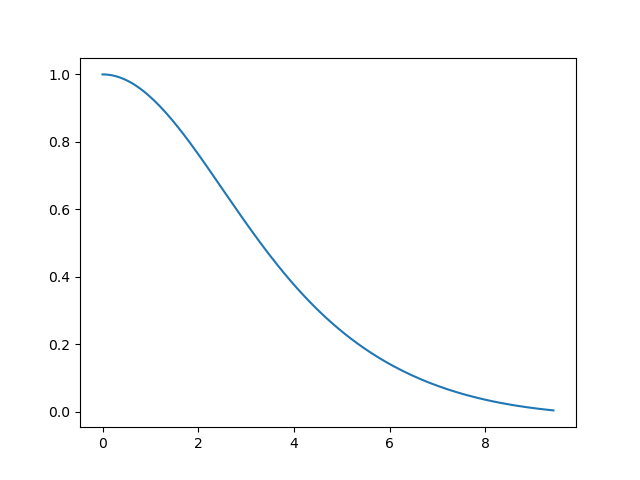
\includegraphics[width=0.78\textwidth]{plot_SW_J1J2_magform_1D.png}
\caption{Magnetic form factor yang digunakan script $J_1$--$J_2$. Pada $g=2$, kurva sama dengan $j_0(q)$ dan turun dari sekitar satu pada $q=0$ menuju nol pada momentum besar. Sumbu horizontal gambar ini adalah $q$ mentah, bukan $q/(2\pi)$.}
\label{fig:j1j2-form}
\end{figure}

\subsection{Dispersi dan bobot mode}

\begin{figure}[H]
\centering
\begin{subfigure}[t]{0.49\textwidth}
\centering
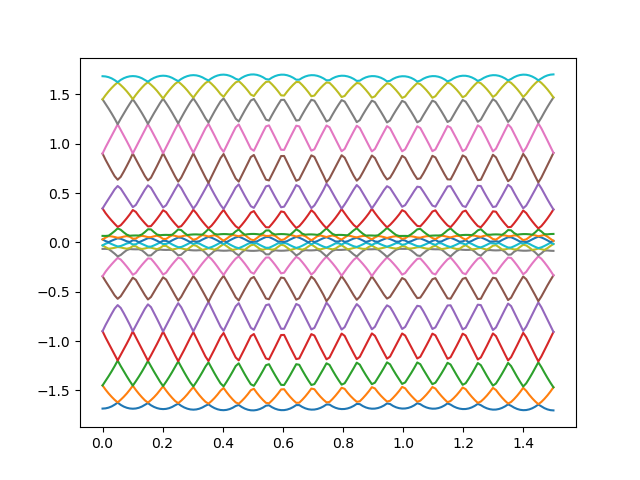
\includegraphics[width=\linewidth]{plot_SW_J1J2_qvsw_1D.png}
\caption{Seluruh eigenvalue terhadap $q/(2\pi)$.}
\end{subfigure}
\hfill
\begin{subfigure}[t]{0.49\textwidth}
\centering
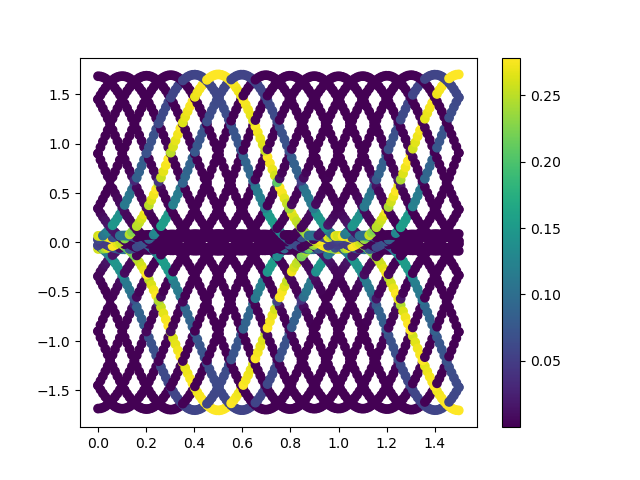
\includegraphics[width=\linewidth]{plot_SW_J1J2_1D.png}
\caption{Eigenvalue yang sama, diwarnai dengan bobot transversal.}
\end{subfigure}
\caption{Spektrum model $J_1$--$J_2$ untuk $M=10$. Nambu space menghasilkan $2M=20$ cabang, tersusun dalam pasangan energi positif dan negatif. Magnetic unit cell yang panjang melipat dispersi ke banyak cabang dalam reduced Brillouin zone.}
\label{fig:j1j2-disp}
\end{figure}

Cabang yang tampak terang pada Gambar~\ref{fig:j1j2-disp} adalah cabang dengan nilai Persamaan~\eqref{eq:scatter-weight} besar. Banyak cabang gelap tetap merupakan eigenmode matematis, tetapi memiliki matrix element kecil untuk operator spin yang dipakai pada plot.

\subsection{Peta intensitas}

\begin{figure}[H]
\centering
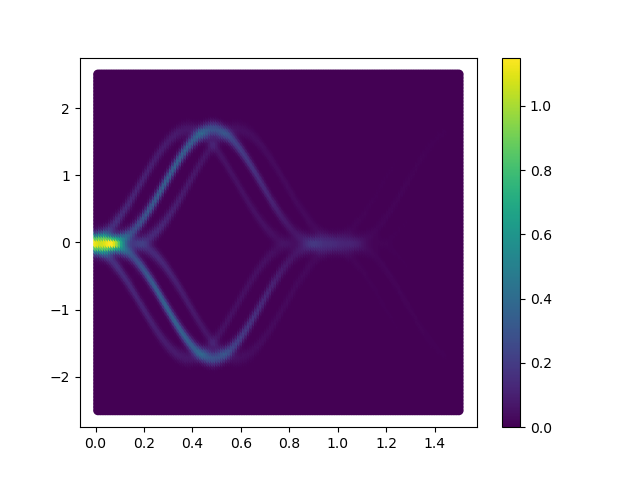
\includegraphics[width=0.80\textwidth]{plot_Intens_SW_J1J2_1D.png}
\caption{Peta intensitas model $J_1$--$J_2$ setelah faktor polarisasi, magnetic form factor, dan Gaussian broadening $\sigma=0.1$. Rentang energi $[-2.5,2.5]$ menampilkan cabang positif dan partner negatif dari representasi Nambu. Untuk perbandingan langsung dengan neutron-energy-loss, bagian $\omega>0$ biasanya yang dipilih.}
\label{fig:j1j2-int}
\end{figure}

Intensitas kuat di sekitar $q=0$ dan $\omega=0$ berasal dari mode berenergi rendah serta tumpang tindih Gaussian. Pada momentum lebih besar, form factor mengurangi bobot, sehingga cabang kanan lebih redup dibanding bagian kiri meskipun eigenvalue-nya tetap ada.

\section{Hasil model \texorpdfstring{$J_1$--$D$}{J1--D}}

\subsection{Dispersi dan bobot mode}

\begin{figure}[H]
\centering
\begin{subfigure}[t]{0.49\textwidth}
\centering
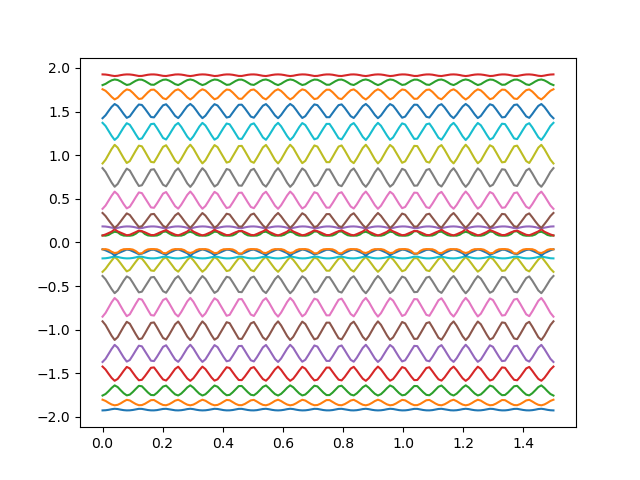
\includegraphics[width=\linewidth]{plot_SW_J1DM_qvsw_1D.png}
\caption{Seluruh eigenvalue terhadap $q/(2\pi)$.}
\end{subfigure}
\hfill
\begin{subfigure}[t]{0.49\textwidth}
\centering
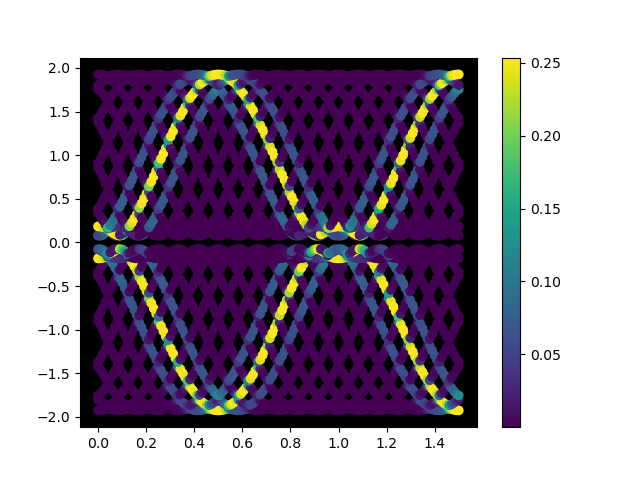
\includegraphics[width=\linewidth]{plot_SW_J1DM_1D.png}
\caption{Eigenvalue dengan bobot transversal sebagai warna.}
\end{subfigure}
\caption{Spektrum model $J_1$--$D$ untuk $M=12$. Terdapat $2M=24$ cabang Nambu. DMI memilih chirality spiral dan memasukkan coupling antisymmetric pada matriks dinamik.}
\label{fig:j1dm-disp}
\end{figure}

Struktur berulang berasal dari kombinasi periodicity reciprocal lattice dan band folding oleh magnetic unit cell 12-sublattice. Pada scatter plot, hanya sebagian kecil cabang yang membawa spectral weight besar.

\subsection{Peta intensitas}

\begin{figure}[H]
\centering
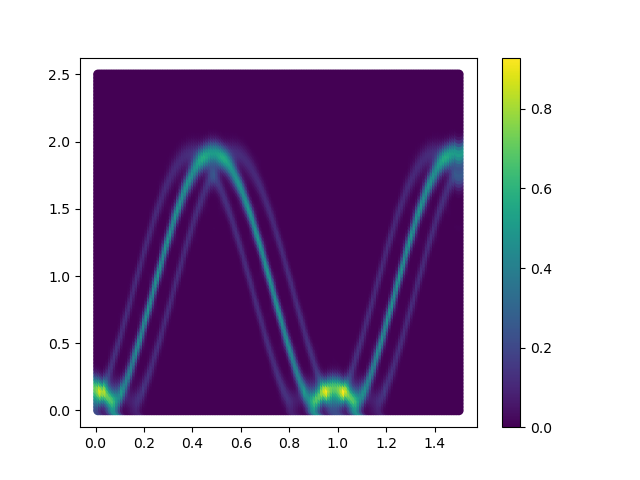
\includegraphics[width=0.80\textwidth]{plot_Intens_SW_J1DM_1D.png}
\caption{Peta intensitas positif model $J_1$--$D$ untuk $\omega\in[0,2.5]$ dengan Gaussian broadening $\sigma=0.08$. Peta menggunakan faktor polarisasi untuk momentum transfer sepanjang $z$ dan tidak memasukkan magnetic form factor tambahan.}
\label{fig:j1dm-int}
\end{figure}

Puncak terang mengikuti cabang eigenvalue positif yang memiliki bobot $S_n^{\alpha\beta}$ besar. Karena peta hanya memakai $\omega\ge0$, partner negatif tidak terlihat, berbeda dari peta $J_1$--$J_2$ pada Gambar~\ref{fig:j1j2-int}.

\section{Hubungan langsung antara teori dan script}

\begin{table}[H]
\centering
\caption{Pemetaan objek teori ke implementasi Julia.}
\begin{tabular}{>{\raggedright\arraybackslash}p{0.27\textwidth}
                >{\raggedright\arraybackslash}p{0.31\textwidth}
                >{\raggedright\arraybackslash}p{0.32\textwidth}}
\toprule
Objek teori & Implementasi & Fungsi fisik\\
\midrule
$R_r=U_r^{-1}$ & \texttt{Uinv(th,phi)} & Rotasi spin lokal ke global\\
$M=\lambda$ & \texttt{M = num\_cell*lmbda} & Jumlah sublattice dalam magnetic cell\\
$L_J$ & \texttt{Lexc}, \texttt{Lexc02} & Exchange nearest dan next-nearest\\
$L_{\mathrm{DM}}$ & \texttt{Ldm} & DMI sepanjang sumbu $y$\\
$\eta$ & \texttt{Ni} & Metric komutasi bosonik\\
$\varepsilon_n,v_n$ & \texttt{eigvals}, \texttt{eigvecs} & Energi dan eigenvector mode\\
$W_{r\alpha n}$ & \texttt{Wra} & Amplitudo fluktuasi spin global\\
$S_n^{\alpha\beta}$ & \texttt{Sab} & Tensor bobot mode\\
$P_{\alpha\beta}$ & \texttt{fac} & Polarization projector\\
$I(q,\omega)$ & \texttt{Sqw} & Peta intensitas ter-broaden\\
\bottomrule
\end{tabular}
\end{table}

Alur numeriknya dapat diringkas sebagai berikut.
\begin{enumerate}
  \item Tetapkan $J_1,J_2$ atau $J_1,D$, pitch $Q$, $S$, dan $M$.
  \item Bangun $\theta_r=(r-1)Q$, $\phi_r=0$, dan $R_r$.
  \item Untuk setiap $q$, isi normal dan pairing block dari seluruh bond.
  \item Bentuk metric $\eta$ dan diagonalize dynamic matrix bosonik.
  \item Bangun $W_{r\alpha n}$ dan $S_n^{\alpha\beta}$ dari eigenvector.
  \item Plot semua eigenvalue untuk grafik $q$--$\omega$.
  \item Gunakan bobot transversal untuk scatter berwarna.
  \item Kontraksikan $S^{\alpha\beta}$ dengan polarization projector, form factor, dan Gaussian untuk memperoleh $I(q,\omega)$.
\end{enumerate}

\section{Pemeriksaan dan batas interpretasi}

Grafik yang dimasukkan adalah keluaran aktual script. Beberapa pemeriksaan berikut diperlukan sebelum hasil dipakai sebagai prediksi kuantitatif eksperimen.

\begin{enumerate}
  \item \textbf{Stationarity.} Pastikan seluruh linear residual $\lambda_r$ bernilai nol untuk pitch yang dipilih.
  \item \textbf{Hermiticity dan pairing symmetry.} Periksa
  \begin{equation}
  \mA(q)^\dagger=\mA(q),
  \qquad
  \Delta(q)^T=\Delta(-q).
  \end{equation}
  \item \textbf{Paraunitary normalization.} Eigenvector bosonik harus dinormalisasi dengan metric $\eta$, bukan norm Euclidean biasa. Ini penting untuk intensitas.
  \item \textbf{Posisi sublattice.} Structure factor eksperimen umumnya memerlukan fase
  \begin{equation}
  \ee^{\ii\vq\cdot(\bm\tau_r-\bm\tau_s)}
  \end{equation}
  pada penjumlahan $r,s$. Persamaan~\eqref{eq:Sab-code} mereproduksi script saat ini, yang belum memasukkan fase basis tersebut secara eksplisit.
  \item \textbf{Titik $q=0$.} Projector~\eqref{eq:polarization} mengandung $q_\alpha q_\beta/q^2$ dan tidak terdefinisi tepat pada $q=0$. Program sebaiknya memakai limit arah $q\to0$ atau melewati titik tersebut.
  \item \textbf{Form factor.} Cross section neutron standar memakai $|f(q)|^2$, sedangkan script $J_1$--$J_2$ saat ini memakai $f(q)$ satu kali.
  \item \textbf{Detailed balance.} Untuk temperatur hingga, sertakan $1+n_B(\omega)$ pada energy-loss dan $n_B(|\omega|)$ pada energy-gain.
  \item \textbf{Second-neighbor block.} Pada script $J_1$--$J_2$, assignment reverse matrix untuk \texttt{Lexc02} dan wrap-around indeks second neighbor perlu diaudit. Salah satu assignment menggunakan \texttt{conj(Lexc[r,sr])} alih-alih \texttt{conj(Lexc02[r,sr])}.
\end{enumerate}

Dengan pemeriksaan tersebut, alur dari Hamiltonian ke grafik menjadi bukan hanya reproduktif, tetapi juga siap dikembangkan menuju perbandingan neutron-scattering yang kuantitatif.

\section{Kesimpulan}

Teori dimulai dari interaksi spin, tetapi grafik akhir memerlukan seluruh rantai transformasi:
\begin{equation}
\boxed{
\begin{aligned}
H_{\mathrm{spin}}
&\longrightarrow
\text{ground state spiral}
\longrightarrow R_r
\longrightarrow
\text{Holstein--Primakoff}\\
&\longrightarrow
\mH_{\mathrm{BdG}}(q)
\longrightarrow
\{\varepsilon_n(q),v_n(q)\}
\longrightarrow
S^{\alpha\beta}(q,\omega)
\longrightarrow I(q,\omega).
\end{aligned}}
\end{equation}

Model $J_1$--$J_2$ menghasilkan spiral karena kompetisi exchange nearest dan next-nearest, dengan $\cos Q=-J_1/(4J_2)$. Model $J_1$--$D$ menghasilkan spiral chiral karena kompetisi exchange dan DMI, dengan $D=J_1\tan Q$. Magnetic unit cell dengan $M=10$ atau $M=12$ melipat spektrum menjadi $2M$ cabang Nambu. Eigenvalue menentukan posisi cabang, sedangkan eigenvector, polarization projector, form factor, dan broadening menentukan cabang mana yang benar-benar tampak terang pada peta intensitas.

\begin{thebibliography}{9}

\bibitem{semiklasik}
\emph{Notes Spinwave Semiklasik}, catatan internal, bagian model Heisenberg, persamaan gerak, feromagnet, anisotropi, dan antiferomagnet.

\bibitem{kuantum}
\emph{Notes Spinwave Kuantum}, catatan internal, bagian operator tangga, satu spin flip, state momentum, dan transformasi Fourier.

\bibitem{hamiltonian}
\emph{Hamiltonian}, catatan internal, derivasi rotasi lokal, Holstein--Primakoff, exchange, anisotropi, DMI, medan, dan matriks $V^\dagger LV$.

\bibitem{j1j2code}
\texttt{SW\_J1J2\_1D.jl}, implementasi Julia untuk rantai spiral $J_1$--$J_2$ dan peta intensitas.

\bibitem{dmcode}
\texttt{SW\_wDM\_1D.jl}, implementasi Julia untuk rantai spiral $J_1$--$D$ dan peta intensitas.

\end{thebibliography}

\end{document}
